% Options for packages loaded elsewhere
\PassOptionsToPackage{unicode}{hyperref}
\PassOptionsToPackage{hyphens}{url}
\PassOptionsToPackage{dvipsnames,svgnames,x11names}{xcolor}
\documentclass[
  11pt,
  fontset=fandol]{ctexart}
\usepackage{xcolor}
\usepackage{amsmath,amssymb}
\setcounter{secnumdepth}{-\maxdimen} % remove section numbering
\usepackage{iftex}
\ifPDFTeX
  \usepackage[T1]{fontenc}
  \usepackage[utf8]{inputenc}
  \usepackage{textcomp} % provide euro and other symbols
\else % if luatex or xetex
  \usepackage{unicode-math} % this also loads fontspec
  \defaultfontfeatures{Scale=MatchLowercase}
  \defaultfontfeatures[\rmfamily]{Ligatures=TeX,Scale=1}
\fi
\usepackage{lmodern}
\ifPDFTeX\else
  % xetex/luatex font selection
    \setmainfont[BoldFont=texgyrepagella-bold.otf,ItalicFont=texgyrepagella-italic.otf,BoldItalicFont=texgyrepagella-bolditalic.otf]{texgyrepagella-regular.otf}
    \setsansfont[BoldFont=texgyreheros-bold.otf,ItalicFont=texgyreheros-italic.otf,BoldItalicFont=texgyreheros-bolditalic.otf]{texgyreheros-regular.otf}
    \setmonofont[]{lmmono10-regular.otf}
\fi
% Use upquote if available, for straight quotes in verbatim environments
\IfFileExists{upquote.sty}{\usepackage{upquote}}{}
\IfFileExists{microtype.sty}{% use microtype if available
  \usepackage[]{microtype}
  \UseMicrotypeSet[protrusion]{basicmath} % disable protrusion for tt fonts
}{}
\makeatletter
\@ifundefined{KOMAClassName}{% if non-KOMA class
  \IfFileExists{parskip.sty}{%
    \usepackage{parskip}
  }{% else
    \setlength{\parindent}{0pt}
    \setlength{\parskip}{6pt plus 2pt minus 1pt}}
}{% if KOMA class
  \KOMAoptions{parskip=half}}
\makeatother
\usepackage{color}
\usepackage{fancyvrb}
\newcommand{\VerbBar}{|}
\newcommand{\VERB}{\Verb[commandchars=\\\{\}]}
\DefineVerbatimEnvironment{Highlighting}{Verbatim}{commandchars=\\\{\}}
% Add ',fontsize=\small' for more characters per line
\newenvironment{Shaded}{}{}
\newcommand{\AlertTok}[1]{\textcolor[rgb]{1.00,0.00,0.00}{\textbf{#1}}}
\newcommand{\AnnotationTok}[1]{\textcolor[rgb]{0.38,0.63,0.69}{\textbf{\textit{#1}}}}
\newcommand{\AttributeTok}[1]{\textcolor[rgb]{0.49,0.56,0.16}{#1}}
\newcommand{\BaseNTok}[1]{\textcolor[rgb]{0.25,0.63,0.44}{#1}}
\newcommand{\BuiltInTok}[1]{\textcolor[rgb]{0.00,0.50,0.00}{#1}}
\newcommand{\CharTok}[1]{\textcolor[rgb]{0.25,0.44,0.63}{#1}}
\newcommand{\CommentTok}[1]{\textcolor[rgb]{0.38,0.63,0.69}{\textit{#1}}}
\newcommand{\CommentVarTok}[1]{\textcolor[rgb]{0.38,0.63,0.69}{\textbf{\textit{#1}}}}
\newcommand{\ConstantTok}[1]{\textcolor[rgb]{0.53,0.00,0.00}{#1}}
\newcommand{\ControlFlowTok}[1]{\textcolor[rgb]{0.00,0.44,0.13}{\textbf{#1}}}
\newcommand{\DataTypeTok}[1]{\textcolor[rgb]{0.56,0.13,0.00}{#1}}
\newcommand{\DecValTok}[1]{\textcolor[rgb]{0.25,0.63,0.44}{#1}}
\newcommand{\DocumentationTok}[1]{\textcolor[rgb]{0.73,0.13,0.13}{\textit{#1}}}
\newcommand{\ErrorTok}[1]{\textcolor[rgb]{1.00,0.00,0.00}{\textbf{#1}}}
\newcommand{\ExtensionTok}[1]{#1}
\newcommand{\FloatTok}[1]{\textcolor[rgb]{0.25,0.63,0.44}{#1}}
\newcommand{\FunctionTok}[1]{\textcolor[rgb]{0.02,0.16,0.49}{#1}}
\newcommand{\ImportTok}[1]{\textcolor[rgb]{0.00,0.50,0.00}{\textbf{#1}}}
\newcommand{\InformationTok}[1]{\textcolor[rgb]{0.38,0.63,0.69}{\textbf{\textit{#1}}}}
\newcommand{\KeywordTok}[1]{\textcolor[rgb]{0.00,0.44,0.13}{\textbf{#1}}}
\newcommand{\NormalTok}[1]{#1}
\newcommand{\OperatorTok}[1]{\textcolor[rgb]{0.40,0.40,0.40}{#1}}
\newcommand{\OtherTok}[1]{\textcolor[rgb]{0.00,0.44,0.13}{#1}}
\newcommand{\PreprocessorTok}[1]{\textcolor[rgb]{0.74,0.48,0.00}{#1}}
\newcommand{\RegionMarkerTok}[1]{#1}
\newcommand{\SpecialCharTok}[1]{\textcolor[rgb]{0.25,0.44,0.63}{#1}}
\newcommand{\SpecialStringTok}[1]{\textcolor[rgb]{0.73,0.40,0.53}{#1}}
\newcommand{\StringTok}[1]{\textcolor[rgb]{0.25,0.44,0.63}{#1}}
\newcommand{\VariableTok}[1]{\textcolor[rgb]{0.10,0.09,0.49}{#1}}
\newcommand{\VerbatimStringTok}[1]{\textcolor[rgb]{0.25,0.44,0.63}{#1}}
\newcommand{\WarningTok}[1]{\textcolor[rgb]{0.38,0.63,0.69}{\textbf{\textit{#1}}}}
\usepackage{longtable,booktabs,array}
\usepackage{calc} % for calculating minipage widths
% Correct order of tables after \paragraph or \subparagraph
\usepackage{etoolbox}
\makeatletter
\patchcmd\longtable{\par}{\if@noskipsec\mbox{}\fi\par}{}{}
\makeatother
% Allow footnotes in longtable head/foot
\IfFileExists{footnotehyper.sty}{\usepackage{footnotehyper}}{\usepackage{footnote}}
\makesavenoteenv{longtable}
\usepackage{graphicx}
\makeatletter
\newsavebox\pandoc@box
\newcommand*\pandocbounded[1]{% scales image to fit in text height/width
  \sbox\pandoc@box{#1}%
  \Gscale@div\@tempa{\textheight}{\dimexpr\ht\pandoc@box+\dp\pandoc@box\relax}%
  \Gscale@div\@tempb{\linewidth}{\wd\pandoc@box}%
  \ifdim\@tempb\p@<\@tempa\p@\let\@tempa\@tempb\fi% select the smaller of both
  \ifdim\@tempa\p@<\p@\scalebox{\@tempa}{\usebox\pandoc@box}%
  \else\usebox{\pandoc@box}%
  \fi%
}
% Set default figure placement to htbp
\def\fps@figure{htbp}
\makeatother
\setlength{\emergencystretch}{3em} % prevent overfull lines
\providecommand{\tightlist}{%
  \setlength{\itemsep}{0pt}\setlength{\parskip}{0pt}}
% Portable CJK typography: ctex + the open Fandol font family.
\usepackage{geometry}
\geometry{a4paper,left=24mm,right=24mm,top=25mm,bottom=25mm,headheight=15pt}
\usepackage{xcolor}
\definecolor{inkblue}{HTML}{254B62}
\definecolor{muted}{HTML}{657681}
\usepackage{setspace}
\setstretch{1.42}
\setlength{\parindent}{2em}
\setlength{\parskip}{0.28em}
\setlength{\emergencystretch}{3em}
\ctexset{
  section={format=\Large\sffamily\bfseries\color{inkblue},beforeskip=1.7em,afterskip=.8em},
  subsection={format=\large\sffamily\bfseries\color{inkblue},beforeskip=1.3em,afterskip=.6em}
}
\usepackage{fancyhdr}
\pagestyle{fancy}
\fancyhf{}
\fancyhead[L]{\small\sffamily\color{muted}软件仓库管理 · 南京大学 GSE 2026}
\fancyhead[R]{\small\sffamily\color{muted}课程讲义}
\fancyfoot[C]{\small\color{muted}\thepage}
\renewcommand{\headrulewidth}{0.3pt}
\renewcommand{\footrulewidth}{0pt}
\usepackage{titling}
\pretitle{\begin{center}\LARGE\sffamily\bfseries\color{inkblue}}
\posttitle{\par\end{center}\vskip .8em}
\predate{\begin{center}}
\postdate{\end{center}}
\setlength{\droptitle}{-2em}
\renewcommand{\maketitle}{%
  \begin{center}
  {\LARGE\sffamily\bfseries\color{inkblue}\thetitle\par}
  \vspace{5mm}
  {\small\sffamily\color{muted}南京大学 · 生成式软件工程 · 第 3 讲}
  \end{center}\vspace{4mm}\thispagestyle{fancy}}
\usepackage{needspace}
\usepackage{fvextra}
\DefineVerbatimEnvironment{Highlighting}{Verbatim}{breaklines,commandchars=\\\{\},fontsize=\small,frame=single,rulecolor=\color{muted},framesep=8pt}
\AtBeginDocument{\hypersetup{colorlinks=true,linkcolor=inkblue,urlcolor=inkblue,bookmarksopen=true}}
\AtBeginDocument{\urlstyle{same}}
\widowpenalty=10000
\clubpenalty=10000
\usepackage{bookmark}
\IfFileExists{xurl.sty}{\usepackage{xurl}}{} % add URL line breaks if available
\urlstyle{same}
\hypersetup{
  pdftitle={软件仓库管理：从项目快照到 AI 协作},
  colorlinks=true,
  linkcolor={Maroon},
  filecolor={Maroon},
  citecolor={Blue},
  urlcolor={Blue},
  pdfcreator={LaTeX via pandoc}}

\title{软件仓库管理：从项目快照到 AI 协作}
\author{}
\date{}

\begin{document}
\maketitle

课程：南京大学《生成式软件工程》2026 年第 3 讲；主讲：蒋炎岩。

视频：\url{https://www.bilibili.com/video/BV1kybV6DE47/}，时长 1:40:14。

本文依据完整原视频、本地音轨转录、选定画面及官方讲义重组。配图来自本次实际下载的视频，均给出来源时间窗口；音频转录采用真实的
20
秒窗口，时间戳不代表逐字强制对齐。本文是经过主题覆盖审查的学习讲义，不是逐字稿，也不声称逐帧检查全部视频。命令示例凡属编辑补充均明确标注。

\section{学习目标}\label{ux5b66ux4e60ux76eeux6807}

读完本讲，应能解释项目为什么需要快照，区分工作区、暂存区与历史，判断一次提交的边界，并说明
AI 生成能力提高后为什么仍需要架构设计、验证和版本管理。

\section{开场：AI
增强执行力，为什么仍然要学基础}\label{ux5f00ux573aai-ux589eux5f3aux6267ux884cux529bux4e3aux4ec0ux4e48ux4ecdux7136ux8981ux5b66ux57faux7840}

开场延续前两讲：把 AI 放进真实生活流程，可以把反复执行的步骤沉淀为
skills。但``能够执行''不等于``已经理解人的意图''。同样一句``做一个好用的应用''，不同的人心里可能对应完全不同的界面和使用方式，模型只能根据已有上下文作出选择。

讲师用当时的模型体验、空间推理和 3D
打印案例说明能力进步带来的冲击。这些属于课堂中的个人观察，不能据此推出永久有效的模型排名，更不能把讲师对模型训练路线的猜测改写成厂商事实。

学习操作系统、数据库等基础仍有现实价值：这些知识提供接口、状态、并发和约束的概念，使人能够提出更准确的问题，也能识别方案的不足。基础知识会影响我们向
AI
提什么要求、允许什么取舍，以及怎样判断结果，而不只是影响能否亲手敲出代码。

\section{1.
为什么只有一个项目目录还不够}\label{ux4e3aux4ec0ux4e48ux53eaux6709ux4e00ux4e2aux9879ux76eeux76eeux5f55ux8fd8ux4e0dux591f}

软件项目通常以目录的形式出现：代码实现行为，文档表达需求与约定，测试描述可以检查的要求，配置和构建脚本决定如何运行。保留当前目录可以保存当下的工作，却不能自动回答``昨天能运行的版本在哪里''。

复制``作业-v1''\,``作业-v2''是一种朴素的版本管理方法。它能留下旧文件，但版本关系需要人工记忆。两个人分别修改同一份代码后，文件应该怎样合并？只恢复旧代码却留下新配置，是否仍是一个能运行的项目？这些问题表明，需要管理的是完整项目状态及其变化关系。

Git 将这些状态组织成可回查的历史。它并不要求先使用
GitHub：本地仓库负责记录版本，GitHub 等平台负责托管以及围绕
issue、审查和发布进行协作。

本章小结：版本管理让项目保留可理解的过去，为恢复、比较和协作提供基础。

\par\addvspace{1em}\noindent\begin{minipage}{\linewidth}\centering

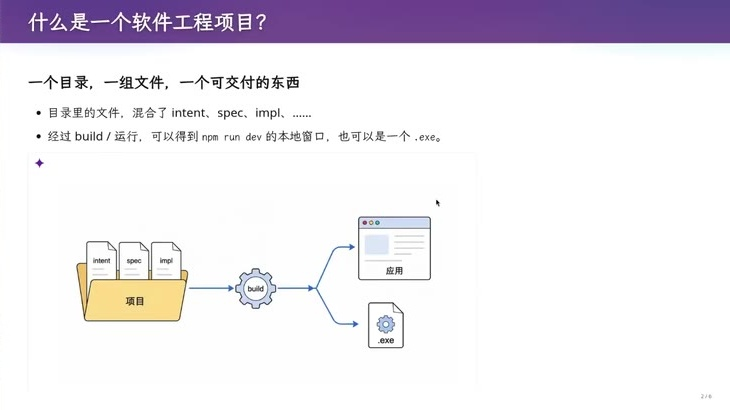
\includegraphics[width=0.94\linewidth,height=8.5cm,keepaspectratio]{notes/fig_project.jpg}

\textbf{项目把意图、规格与实现组织为可交付产物}

\raggedright\footnotesize\color{muted}

画面证据：原视频
10:00--10:15，\href{https://www.bilibili.com/video/BV1kybV6DE47/?t=600}{回看项目目录示意}。课件把
intent、spec、impl 放在同一个项目目录中，通过构建得到应用或可执行文件。

\end{minipage}\par\addvspace{1em}

\subsection{从 U
盘与压缩包，推导出版本管理}\label{ux4ece-u-ux76d8ux4e0eux538bux7f29ux5305ux63a8ux5bfcux51faux7248ux672cux7ba1ux7406}

课堂先讲代码保存在 U
盘、用邮件发压缩包的经历，再从``我想回到昨天的状态''推导出工具需求。复制目录能暂时满足回溯，但很难表达谁从哪个版本出发、哪些文件应该成组变化、两人的工作怎样汇合。

从需求出发，可以先想出一个能列出版本、切换状态的简单系统，再逐渐增加分支和合并。课堂讲述
RCS、CVS、SVN、BitKeeper 与 Git
的背景，是为了说明工具由真实协作问题推动。学习时应区分``用于理解的简化模型''与某个工具全部版本的实际存储细节，不能只凭一句``快照''或``差分''推断其所有实现。

\section{2.
快照如何构成历史}\label{ux5febux7167ux5982ux4f55ux6784ux6210ux5386ux53f2}

Git
在逻辑上记录项目快照。快照描述被跟踪文件在某个时刻的内容与目录位置；提交进一步关联说明、作者和父提交。沿父提交回溯，就能看到项目如何演变。

完整快照不意味着每次物理复制所有文件。相同内容可以复用，目录对象引用已有内容，因此少量修改不需要重复保存所有未变的部分。理解这个模型，可以避免把
Git 仅看成一串压缩包。

\Needspace{11\baselineskip}

\begin{longtable}[]{@{}ll@{}}
\toprule\noalign{}
概念 & 承担的作用 \\
\midrule\noalign{}
\endhead
\bottomrule\noalign{}
\endlastfoot
blob & 保存文件内容的字节序列 \\
tree & 组织目录条目、名称及其引用的对象 \\
commit & 关联根目录树、父提交和提交信息 \\
分支 & 指向某个提交的可移动引用 \\
HEAD & 通常标识当前分支，也可以直接指向提交 \\
\end{longtable}

课堂使用可视化工具观察真实仓库对象。这种学习方法的价值在于把``对象''\,``引用''等抽象名词与磁盘中的实际数据联系起来，观察一次操作究竟改变了什么。

本章小结：Git
保存项目状态，也保存状态之间的关系；对象复用使快照可以高效存储。

\subsection{持久化目录树为什么不必复制整个项目}\label{ux6301ux4e45ux5316ux76eeux5f55ux6811ux4e3aux4ec0ux4e48ux4e0dux5fc5ux590dux5236ux6574ux4e2aux9879ux76ee}

设目录中有 A、B 和子目录 D。若只改了 B，新版本需要保存 B
的新内容，以及从 B 到根目录这条路径上发生变化的目录节点；A 和 D
可以继续指向旧对象。旧版本仍可沿旧的引用访问，新版本沿新的引用访问，这就是课堂用来说明持久化数据结构的直觉。

课堂的 \texttt{gitv}
工具不是仅在网页上模拟几个提交，而是读取真实仓库的文件及其原始字节，展示解压后的对象内容。这样可以检查
blob、tree 和 commit
这些名词究竟对应什么。观察对象时还要区分压缩前后大小：磁盘文件字节数、对象头和正文长度是不同量，不能把它们混为同一指标。

\par\addvspace{1em}\noindent\begin{minipage}{\linewidth}\centering

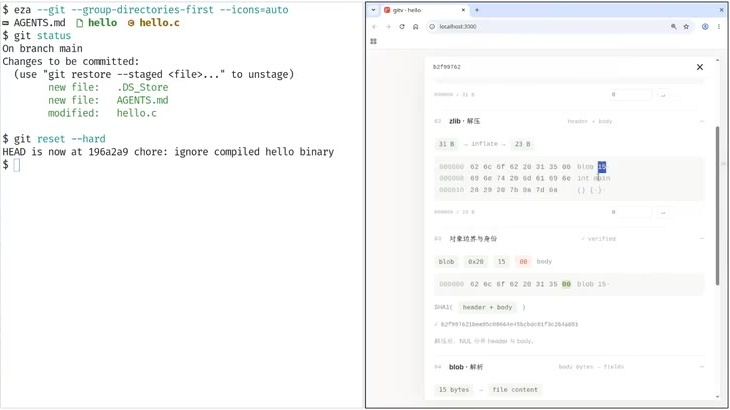
\includegraphics[width=0.94\linewidth,height=8.5cm,keepaspectratio]{notes/fig_git_visual.jpg}

\textbf{从真实对象文件查看 blob 字节与解析结果}

\raggedright\footnotesize\color{muted}

画面证据：72:30--72:45，\href{https://www.bilibili.com/video/BV1kybV6DE47/?t=4350}{回看真实
Git
对象}。右侧展示对象字节及解析，左侧是终端状态；图中命令是演示现场，不是要求读者照做的恢复方案。

\end{minipage}\par\addvspace{1em}

\section{3.
为什么要区分工作区和暂存区}\label{ux4e3aux4ec0ux4e48ux8981ux533aux5206ux5de5ux4f5cux533aux548cux6682ux5b58ux533a}

工作区是正在编辑的文件，暂存区保存下一次提交准备采用的内容，提交历史保存已经记录的快照。暂存区允许开发者组织一次修改，而不是把所有正在探索的内容一次打包。

编辑补充示例：

\begin{Shaded}
\begin{Highlighting}[]
\FunctionTok{git}\NormalTok{ init}
\FunctionTok{git}\NormalTok{ add hello.c}
\FunctionTok{git}\NormalTok{ diff }\AttributeTok{{-}{-}cached}
\FunctionTok{git}\NormalTok{ commit }\AttributeTok{{-}m} \StringTok{"feat: add a minimal hello program"}
\end{Highlighting}
\end{Shaded}

如果执行 \texttt{git\ add\ hello.c} 后又修改了文件，普通
\texttt{git\ commit}
提交的是已暂存的版本。后续编辑仍留在工作区，需要再次暂存才进入这次提交。\texttt{git\ diff}
用于查看未暂存的修改，\texttt{git\ diff\ -\/-cached}
用于查看已暂存的修改。

这也说明为什么不应不经检查就执行
\texttt{git\ add\ .}：它可能把编译产物、临时文件和私人配置一起纳入提交。命令合法，不代表项目选择合理。

\par\addvspace{1em}\noindent\begin{minipage}{\linewidth}\centering

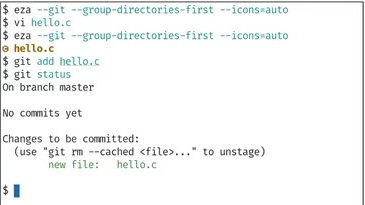
\includegraphics[width=0.94\linewidth,height=8.5cm,keepaspectratio]{notes/fig_init.jpg}

\textbf{执行 git add 后，git status 显示准备提交的 hello.c}

\raggedright\footnotesize\color{muted}

画面证据：37:30--37:45，\href{https://www.bilibili.com/video/BV1kybV6DE47/?t=2250}{回看暂存区状态}。界面明确写着
\texttt{No\ commits\ yet}，但 \texttt{hello.c}
已列在准备提交的变化中；这正好说明暂存与提交是两步。

\end{minipage}\par\addvspace{1em}

本章小结：提交是经过选择和组织的变更；暂存区提供了表达这一选择的位置。

\section{4.
分支、合并与冲突解决了什么问题}\label{ux5206ux652fux5408ux5e76ux4e0eux51b2ux7a81ux89e3ux51b3ux4e86ux4ec0ux4e48ux95eeux9898}

分支让不同工作可以从共同起点向前推进。一个人修改界面，另一个人修改解析器，双方先记录各自的变化，再合并结果。

Git
可以依据共同祖先与双方修改计算合并。当同一段文本出现无法自动决定的变化时，工作区通常会出现冲突标记，展示双方内容。开发者需要理解上下文，把文件改成最终需要的结果，再标记解决并完成提交。

合并成功只说明文本变化得到组合，不说明行为正确。两个分支即使修改不同文件，也可能在接口、配置或业务规则上不兼容，所以还要验证组合后的项目。

官方讲义补充说明了
rebase：它把一串改动重新应用到新的起点，通常会产生新的提交标识。是否可以整理历史取决于协作约定；别人已经依赖的提交不宜随意改写。

本章小结：分支隔离尝试，合并汇合变化；验证负责判断组合后的行为。

\subsection{冲突标记之外，暂存区还记录了什么}\label{ux51b2ux7a81ux6807ux8bb0ux4e4bux5916ux6682ux5b58ux533aux8fd8ux8bb0ux5f55ux4e86ux4ec0ux4e48}

课堂的可视化演示进一步展示了冲突时的
base、ours、theirs：共同基础和两侧内容同时参与判断。工作区中的尖括号标记让人看到冲突，但解决它并不是机械点击``保留我方''；要结合这段代码应实现的行为选择或重新编写结果。

解决冲突后，暂存区中的冲突状态消失，合并提交关联最终目录树与双方父提交。图上多了一个节点只是表象，真正重要的是它表示哪份结果，以及这份结果从哪些历史状态汇合而来。

\par\addvspace{1em}\noindent\begin{minipage}{\linewidth}\centering

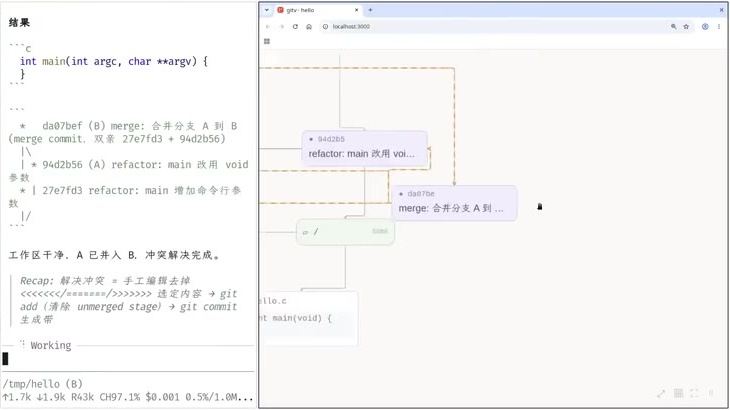
\includegraphics[width=0.94\linewidth,height=8.5cm,keepaspectratio]{notes/fig_merge_visual.jpg}

\textbf{演示结束后的合并提交与分支关系}

\raggedright\footnotesize\color{muted}

画面证据：77:30--77:45，\href{https://www.bilibili.com/video/BV1kybV6DE47/?t=4650}{回看合并结果}。左侧解释解决冲突和生成提交的流程，右侧展示仓库历史关系。

\end{minipage}\par\addvspace{1em}

\section{5.
怎样组织一次有意义的提交}\label{ux600eux6837ux7ec4ux7ec7ux4e00ux6b21ux6709ux610fux4e49ux7684ux63d0ux4ea4}

课程最值得记住的工程原则是，把项目看作由小而完整的变更推进的一系列快照。这里的``小''首先指目的清楚，而非行数少。实现一个功能可能涉及代码、测试和文档，它们共同服务同一意图，可以组成一次完整提交。

相反，修复错误时顺手重排整个项目，会混合不同目的。将来出现故障，读者难以判断哪些变化相关，也难以单独撤销。保持提交边界清楚，可以降低审查、恢复与定位问题的成本。

提交说明应补充 diff 没有直接表达的意图。只有 \texttt{update}
或``做了些东西''，无法帮助后来的人理解变化。标题概括行为，正文解释动机、约束和取舍；具体格式服从项目约定。

编辑补充示例：

\begin{Shaded}
\begin{Highlighting}[]
\NormalTok{fix(parser): accept repeated spaces between arguments}

\NormalTok{Ignore extra spaces between arguments while preserving spaces inside quotes.}
\end{Highlighting}
\end{Shaded}

Conventional Commits 提供 \texttt{type(scope):\ description}
的一种组织方式，但格式正确不等于说明充分。代码能否构建、相关测试能否通过，同样影响这次提交能否成为可靠的历史检查点。

\par\addvspace{1em}\noindent\begin{minipage}{\linewidth}\centering

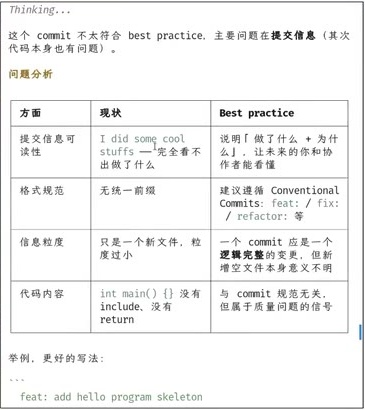
\includegraphics[width=0.94\linewidth,height=8.5cm,keepaspectratio]{notes/fig_commit_review.jpg}

\textbf{Agent 对课堂提交的说明、格式和信息粒度进行检查}

\raggedright\footnotesize\color{muted}

画面证据：40:00--40:15，\href{https://www.bilibili.com/video/BV1kybV6DE47/?t=2400}{回看提交审查}。示例提交的主要问题是说明没有信息量；图中的规范建议服务于读者理解，不意味着所有仓库必须使用完全相同的格式。

\end{minipage}\par\addvspace{1em}

\subsection{空提交为什么存在，又为什么不应滥用}\label{ux7a7aux63d0ux4ea4ux4e3aux4ec0ux4e48ux5b58ux5728ux53c8ux4e3aux4ec0ux4e48ux4e0dux5e94ux6ee5ux7528}

课堂通过没有文件变化的提交说明，提交不仅包含目录树，也有说明等元信息。有时可以借空提交触发自动流程或表达一个明确的工程事件，但如果大量空提交没有可解释目的，历史会增加噪声。发布标记也可以通过
tag 表达，选哪种形式取决于项目约定。

课堂还让 Agent 整理实验历史：它先注意到仓库没有
remote，再处理先前不合理的提交。这一细节体现了历史重写与协作的关系。别人已经基于某段历史工作时，改写它会改变共同参照，不能只因为``整理后看起来漂亮''就忽略依赖关系。

本章小结：好的提交边界让变化可以解释，好的说明让后来的人知道为什么要保留它。

\section{6.
什么应该进入仓库}\label{ux4ec0ux4e48ux5e94ux8be5ux8fdbux5165ux4ed3ux5e93}

仓库保存共同维护的项目状态，不必保存工作目录里出现的一切。编译产物和日志通常能由源码及工具重新生成，不适合每次提交；机器绝对路径和个人编辑器偏好也可能让他人无法复现。

\Needspace{11\baselineskip}

\begin{longtable}[]{@{}ll@{}}
\toprule\noalign{}
文件类型 & 判断依据 \\
\midrule\noalign{}
\endhead
\bottomrule\noalign{}
\endlastfoot
源码、测试、构建说明 & 通常是共同维护的项目内容 \\
编译产物、运行日志 & 通常忽略，防止膨胀及无意义冲突 \\
私人路径和临时文件 & 通常排除，避免依赖个人机器 \\
凭据与 API key & 不进入版本历史 \\
依赖锁文件或生成头文件 & 依据复现需求、工具链和团队约定决定 \\
\end{longtable}

``生成文件一律不提交''过于简单。锁文件可以固定依赖版本，某些生成头文件可以减少使用者安装额外工具链的负担。关键问题是为什么共享它，以及怎样保持一致。

官方讲义提醒：\texttt{.gitignore}
不会让已经跟踪的文件自动退出历史。误提交密钥后，仅删掉当前文件不能消除旧版本中的泄露，应按凭据类型处理失效、轮换及历史清理。

本章小结：根据文件在项目中的角色决定是否提交，不按文件名机械判断。

\par\addvspace{1em}\noindent\begin{minipage}{\linewidth}\centering

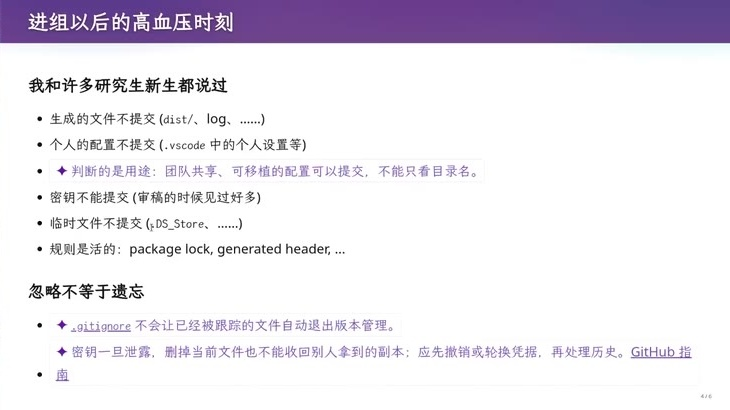
\includegraphics[width=0.94\linewidth,height=8.5cm,keepaspectratio]{notes/fig_exclude.jpg}

\textbf{课件列举生成文件、个人配置、密钥及规则的例外}

\raggedright\footnotesize\color{muted}

画面证据：57:30--57:45，\href{https://www.bilibili.com/video/BV1kybV6DE47/?t=3450}{回看文件选择规则}。课件同时强调规则依用途判断，以及忽略文件不等于抹除已有历史。

\end{minipage}\par\addvspace{1em}

\subsection{从规则命名理解工程上的判断}\label{ux4eceux89c4ux5219ux547dux540dux7406ux89e3ux5de5ux7a0bux4e0aux7684ux5224ux65ad}

课堂比较 \texttt{{[}TYPO-CHECK{]}\ Docs\ should\ be\ typo-free}
与小写标识的写法。方括号中的内容承担固定规则名的角色，后半句承担自然语言解释的角色；两者视觉上可区分，规则也更便于被引用。这个分析解释了为何有人偏好大写，并不推出``大写永远更好''。

如果工具要求小写，或项目一直使用小写，一致性可能比局部醒目更重要。细节学习的目的，是把模糊直觉还原成角色、约束和取舍，而不是积累没有前提的口号。

\par\addvspace{1em}\noindent\begin{minipage}{\linewidth}\centering

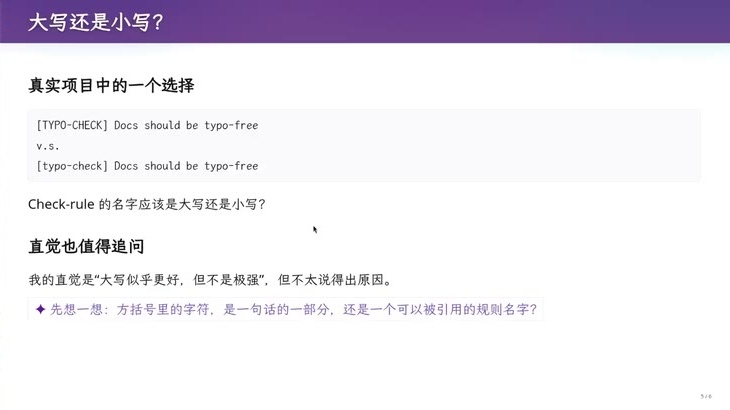
\includegraphics[width=0.94\linewidth,height=8.5cm,keepaspectratio]{notes/fig_rule_name.jpg}

\textbf{TYPO-CHECK 与 typo-check 的规则命名对比}

\raggedright\footnotesize\color{muted}

画面证据：60:00--60:15，\href{https://www.bilibili.com/video/BV1kybV6DE47/?t=3600}{回看规则名讨论}。

\end{minipage}\par\addvspace{1em}

\section{7.
历史如何帮助验证与恢复}\label{ux5386ux53f2ux5982ux4f55ux5e2eux52a9ux9a8cux8bc1ux4e0eux6062ux590d}

及时保存合理的检查点，可以让失败的探索有退路。\texttt{git\ bisect}
利用好版本与坏版本间的检查结果缩小范围，帮助找到引入问题的提交；\texttt{git\ blame}
帮助追溯代码行的来源；\texttt{git\ revert}
则以新提交表达对既有变化的撤销。

这些工具的效果取决于历史质量。如果一个提交混合了许多独立目的，定位到它后仍需拆解；如果大量中间版本无法构建，也会增加二分检查的困难。

GitHub 上的 issue、PR 和检查结果属于平台协作信息，并不自动包含在 Git
的文件历史中。课堂提到的 \texttt{gh}、\texttt{glab} 可以让 Agent
通过命令行连接这些协作步骤。使用平台工具仍要区分本地验证、远端推送、提出合并申请和正式合入。

本章小结：历史不仅用来存档，也可以成为定位、审查和恢复的工具。

\subsection{经常保存，与发布前整理并不矛盾}\label{ux7ecfux5e38ux4fddux5b58ux4e0eux53d1ux5e03ux524dux6574ux7406ux5e76ux4e0dux77dbux76fe}

探索时先保留检查点，可以降低误操作后无处可退的风险；准备交给他人时，再在允许的范围内整理成目的清楚的变化。只存在于工作区的修改没有自动进入提交历史，远端
clone 也不会包含这些未提交内容。

课堂围绕小步提交解释了 bisect、review、revert
的价值：每一步如果可构建、可检查，后续操作就有可靠的判断单位。这是``小提交''的工程意义，而不是把一项完整修改任意拆成许多无法运行的碎片。

\par\addvspace{1em}\noindent\begin{minipage}{\linewidth}\centering

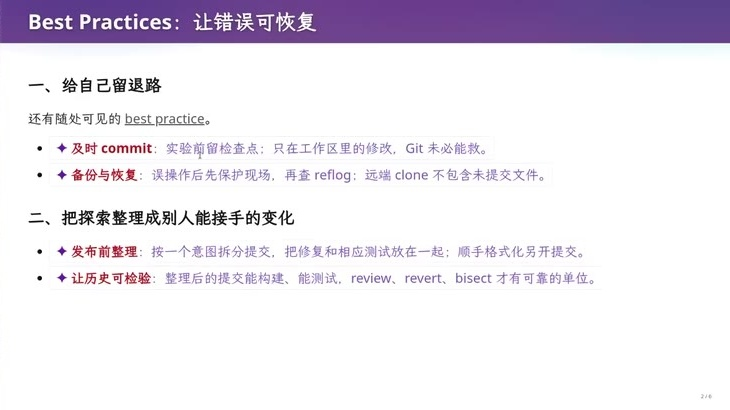
\includegraphics[width=0.94\linewidth,height=8.5cm,keepaspectratio]{notes/fig_best_practice.jpg}

\textbf{检查点、备份与按意图整理历史}

\raggedright\footnotesize\color{muted}

画面证据：90:00--90:15，\href{https://www.bilibili.com/video/BV1kybV6DE47/?t=5400}{回看可恢复的工程实践}。

\end{minipage}\par\addvspace{1em}

\subsection{hooks、CI
与平台工具分工}\label{hooksci-ux4e0eux5e73ux53f0ux5de5ux5177ux5206ux5de5}

Git hooks 可以在提交等事件附近执行检查，CI
可以在集成流程中检查构建与测试。课堂还展示了 Agent 完成任务时发提示音的
hook；它是 Agent 工具的事件机制，与 Git 的 pre-commit hook
不能混成同一个东西。

规则和自动化只能检查已经表达的要求。格式检查通过，不能证明接口设计合理；分支各自测试通过，也不等于组合后的项目通过。\texttt{gh}、\texttt{glab}
把平台中的 issue、评论与 PR 操作连接到工作流程，Git 则继续负责文件版本。

\section{8. AI
能写代码以后，人还要做什么}\label{ai-ux80fdux5199ux4ee3ux7801ux4ee5ux540eux4ebaux8fd8ux8981ux505aux4ec0ux4e48}

课程建议在架构阶段先集中讨论：明确职责、接口和约束，减少相互影响的共享状态，再把边界写成文档、规则与示例。接口稳定后，更多实现细节可以交给
Agent 独立处理。

课堂的编程可视化项目说明了这种做法。通过清晰接口和较少的核心共享状态，组件可以成为相对独立的黑盒，Agent
只需要理解接口，而不必读取所有实现。

实现阶段可以安排多个 Agent
处理相互独立的任务，但并发数量并非质量保证。任务依赖、文件覆盖、接口兼容和集成责任仍需要管理。讲师展示的是个人工作方式，不是所有项目都应遵守的并发上限。

有界面的项目应尽早运行并观察效果。只读``已完成''不能发现按钮位置、交互顺序或文字密度的问题；持续反馈可以尽早纠正设计偏差。

课程结尾提出进一步的问题：当生成速度远超人的理解和验收速度，版本控制与协作方式会遇到什么瓶颈？这节课提出问题，为后续讨论铺垫，不把设想写成已实现的自动化系统。

本章小结：人的贡献更多体现在定义目标、形成设计边界和判断结果，版本管理让探索过程可控。

\subsection{案例：为什么儿童编程环境需要先做好架构}\label{ux6848ux4f8bux4e3aux4ec0ux4e48ux513fux7ae5ux7f16ux7a0bux73afux5883ux9700ux8981ux5148ux505aux597dux67b6ux6784}

讲师展示了面向小学三、四年级学生的编程环境。目标是让孩子尽快看到 Python
程序的效果，而非先学习复杂 IDE
的所有配置。演示把代码、运行轨迹和可视化画面联系起来，拖动进度可以观察不同执行状态。

这样的界面看起来只是几块面板，但背后需要明确接口：程序怎样产生轨迹，轨迹怎样驱动图像，光标和播放位置怎样协调。讲师强调把尽可能多的组件设计成纯函数，把少量跨组件状态集中管理；于是实现组件的
Agent 可以只依赖接口，减少反复阅读其他实现的成本。

\par\addvspace{1em}\noindent\begin{minipage}{\linewidth}\centering

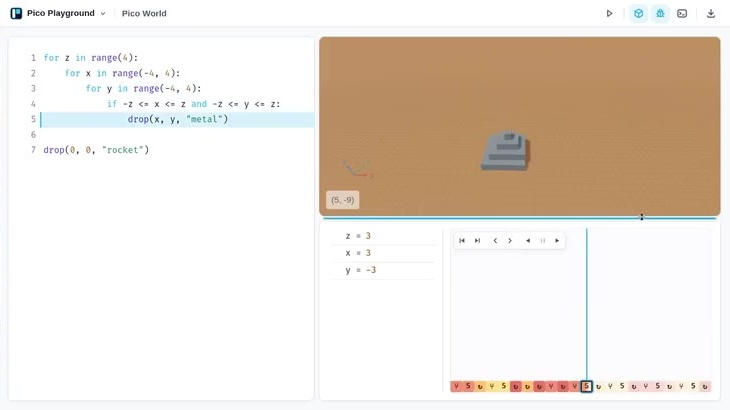
\includegraphics[width=0.94\linewidth,height=8.5cm,keepaspectratio]{notes/fig_playground.jpg}

\textbf{Pico Playground 中的程序、运行轨迹与三维结果}

\raggedright\footnotesize\color{muted}

画面证据：82:30--82:45，\href{https://www.bilibili.com/video/BV1kybV6DE47/?t=4950}{回看编程环境}。本文只说明课堂演示的架构与交互，不声称已独立复现此工具。

\end{minipage}\par\addvspace{1em}

\subsection{多个 Agent
的前提仍是边界清楚}\label{ux591aux4e2a-agent-ux7684ux524dux63d0ux4ecdux662fux8fb9ux754cux6e05ux695a}

进入实现阶段之前，先通过架构讨论形成共同前提，再用 \texttt{AGENTS.md}
记录规则。实现过程中及时观察真实效果、指出不足，让偏差尽快暴露。并行处理边界清楚的任务可以推进工作；不断增加终端数量，却不明确谁负责接口和集成，会把混乱转移到合并阶段。

\par\addvspace{1em}\noindent\begin{minipage}{\linewidth}\centering

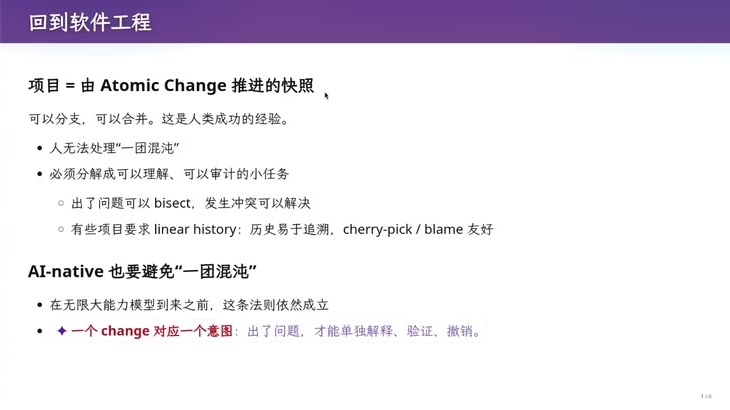
\includegraphics[width=0.94\linewidth,height=8.5cm,keepaspectratio]{notes/fig_atomic.jpg}

\textbf{项目由原子变更推进，以及 AI-native 项目也应避免混沌}

\raggedright\footnotesize\color{muted}

画面证据：95:00--95:15，\href{https://www.bilibili.com/video/BV1kybV6DE47/?t=5700}{回看本讲工程总结}。

\end{minipage}\par\addvspace{1em}

\subsection{结尾的思想实验：当生成速度增长一千倍}\label{ux7ed3ux5c3eux7684ux601dux60f3ux5b9eux9a8cux5f53ux751fux6210ux901fux5ea6ux589eux957fux4e00ux5343ux500d}

最后的课件把``快一千倍''作为放大矛盾的思想实验：如果代码生成极快，而人理解和验收的速度没有跟上，积压的会是等待判断的变更。系统需要回答哪些改动能组合、哪些有依赖、哪些组合后要重新验证。

这里的数字不是一次性能测试结果，也不表示课堂已经实现了一套新版本控制系统。它把问题引向变更组合、并发控制与准入判断，说明今天学习快照、接口和验证概念，仍能帮助理解未来的工具。

\par\addvspace{1em}\noindent\begin{minipage}{\linewidth}\centering


\includegraphics[width=0.94\linewidth,height=8.5cm,keepaspectratio]{notes/fig_future.jpg}

\textbf{关于 Agent 产能与版本控制的结尾思想实验}

\raggedright\footnotesize\color{muted}

画面证据：100:00--100:13，\href{https://www.bilibili.com/video/BV1kybV6DE47/?t=6000}{回看结尾课件}。该画面确实在原视频末尾，本文不据此推断已经发生了后续讨论。

\end{minipage}\par\addvspace{1em}

\section{9. 怎样借助 AI
学习工程知识}\label{ux600eux6837ux501fux52a9-ai-ux5b66ux4e60ux5de5ux7a0bux77e5ux8bc6}

课程反复强调注意力：看到成熟项目时，留意目录、文档和操作反馈。先想自己会如何解决，再比较现成方案；如果对方更好，追问它解决了哪个自己忽略的约束。

这种方法被称为 virtually
implement。它适用于读代码、论文、README，也适用于检查 AI
生成的解释。重点是形成预测并用证据修正理解。

学习 Git 时，可以要求 Agent
在操作前解释将影响哪些文件、暂存内容与历史引用，在操作后展示状态变化。这样每次真实任务都能补充一个概念，而不只是记住一条命令。

\par\addvspace{1em}\noindent\begin{minipage}{\linewidth}\centering


\includegraphics[width=0.94\linewidth,height=8.5cm,keepaspectratio]{notes/fig_learning.jpg}

\textbf{Virtually Implement 的课堂定义与注意细节的方法}

\raggedright\footnotesize\color{muted}

画面证据：22:30--22:45，\href{https://www.bilibili.com/video/BV1kybV6DE47/?t=1350}{回看学习方法}。课堂把它延伸到阅读项目、文档乃至
AI 生成的解释。

\end{minipage}\par\addvspace{1em}

比较成熟项目的 README
也是这种方法的例子。长文档不必然信息充分，短文档也不必然清楚。应该观察读者进入项目时有哪些问题，入口是否能让人迅速找到下一步需要的内容。课堂用路口标识作类比，强调把所需信息放在产生不确定性的地方。

\section{小结与练习}\label{ux5c0fux7ed3ux4e0eux7ec3ux4e60}

项目的演变应能被分解为可理解的变更。快照提供可恢复状态，分支和合并组织协作，清楚的提交边界与验证让历史真正有用。

练习：在一次性练习仓库中，修改文件后先暂存，再修改一次，比较两个
diff；创建两条修改同一行的分支，观察冲突；检查自己的项目中是否存在不应跟踪的产物。让
Agent 先解释预期结果，再执行并核对。

\enlargethispage{3\baselineskip}

\section{来源与许可}\label{ux6765ux6e90ux4e0eux8bb8ux53ef}

\begin{itemize}
\tightlist
\item
  原课程：蒋炎岩，南京大学《生成式软件工程》2026 年第 3 讲，视频
  \url{https://www.bilibili.com/video/BV1kybV6DE47/}。
\item
  \href{https://jyywiki.cn/GSE/2026/lect3.md}{官方讲义《版本管理》}。
\item
  \href{https://github.com/NinZeige/NJU-2026-GSE-Captions/tree/main/release/03-软件仓库管理}{公开字幕整理稿}，来源仓库尚未将本讲标记为完成人工校对。
\item
  原课程与字幕整理来源采用
  \href{https://creativecommons.org/licenses/by-nc/4.0/}{CC BY-NC
  4.0}。本文对相关内容作删减、重排和解释，保留署名并按相同条件提供对应改编内容，不代表讲师或学校认可。
\end{itemize}

核验材料见仓库
\texttt{evidence/}，包含媒体哈希、字幕、配图来源和覆盖表。按 5
分钟窗口抽查并核对 12 幅原图，未作逐字、逐帧全检或课堂工具复现。

\end{document}
